% presentation
\documentclass[compress]{beamer}

% handout
%\documentclass[handout]{beamer}

\usepackage{../mtex,fancyvrb,booktabs}
\usepackage{tikz}
%\usepackage{subfigure}
\usepackage[labelformat=empty]{subcaption}
\captionsetup{compatibility=false}

\author{R. Hielscher}

\title{Misorientation Analysis}
%\subtitle{Chemnitz {\bf{\color{red}M}TEX} Workshop 2015}

\institute{Faculty of Mathematics,\\
	Chemnitz University of Technology, Germany}

\date{{\bf{\color{red}M}TEX} Workshop 2015}



\begin{document}

\begin{frame}
  \maketitle{}
\end{frame}


\section{Misorientations}


\subsection*{Coordinate Transforms}
\label{sec:orientations}


\begin{frame}[fragile]
  \frametitle{Coordinate Transforms}

  \begin{overlayarea}{\textwidth}{8cm}

    Consider a Magnetite grain in cube orientation
    \vspace{-0.2cm}
    \begin{lstlisting}[style=input]
CS_Mag = loadCIF('Magnetite')
O_Mag  = orientation.id(CS_Mag)
   \end{lstlisting}
   \begin{onlyenv}<1>
     \vspace{-0.3cm}
     \begin{lstlisting}[style=output]
CS_Mag = /+crystalSymmetry+/ (show methods, plot)
  mineral : Magnetite
  symmetry: m-3m
  a, b, c : 8.4, 8.4, 8.4

O_Mag = /+orientation+/ (show methods, plot)
  size: 1 x 1
  crystal symmetry : Magnetite (m-3m)
  specimen symmetry: 1

  Bunge Euler angles in degree
  phi1  Phi phi2 Inv.
  0    0    0    0
    \end{lstlisting}
  \end{onlyenv}

  \pause

  Remember, orientations convert crystal into specimen
  coordinates.
  \vspace{-.2cm}
  \begin{lstlisting}[style=input]
r = O_Mag * Miller(1,1,1,CS_Mag)
\end{lstlisting}
  \begin{onlyenv}<2>
\vspace{-.3cm}\begin{lstlisting}[style=output]
r = /+vector3d+/ (show methods, plot)
 size: 1 x 1
         x        y        z
  0.119107 0.119107 0.119107
\end{lstlisting}
  \end{onlyenv}

  \pause

  Take a Hematite grain with orientation
  \vspace{-0.2cm}
  \begin{lstlisting}[style=input]
CS_Hem = loadCIF('Hematite')
O_Hem  = orientation('Euler',...
           135*degree,55*degree,60*degree,CS_Hem)
   \end{lstlisting}
   \begin{onlyenv}<3>
     \vspace{-0.3cm}
     \begin{lstlisting}[style=output]
O_Hem = orientation (show methods, plot)
  size: 1 x 1
  crystal symmetry : Hematite (-3m1, X||a*, Y||b, Z||c)
  specimen symmetry: 1

  Bunge Euler angles in degree
  phi1     Phi    phi2    Inv.
   135 54.7356      60       0
    \end{lstlisting}
  \end{onlyenv}

  \pause

  inverse orientations convert specimen into crystal coordinates
  \vspace{-.2cm}
  \begin{lstlisting}[style=input]
inv(O_Hem) * r
\end{lstlisting}
  \begin{onlyenv}<4>
    \vspace{-.3cm}
    \begin{lstlisting}[style=output]
ans = /+Miller+/ (show methods, plot)
 mineral: Hematite (-3m1, X||a*, Y||b, Z||c)
  h 0
  k 0
  i 0
  l 1
\end{lstlisting}
  \end{onlyenv}
\end{overlayarea}

\end{frame}



\subsection*{Misorientations}
\label{sec:orientations2}

\begin{frame}[fragile]
  \frametitle{Misorientations}

  \begin{overlayarea}{\textwidth}{8cm}

  Hence, $\text{\bf inv}(\mathbf{O\_Hem}) \cdot \mathbf{O\_MAG}$ converts crystal  into
  crystal coordinates
  \begin{lstlisting}[style=input]
inv(O_Hem) * O_Mag * Miller(1,1,1,0,CS_Mag)
  \end{lstlisting}
  \begin{onlyenv}<1>
    \vspace{-.3cm}
    \begin{lstlisting}[style=output]
ans = /+Miller+/ (show methods, plot)
 size: 1 x 1
 mineral: Hematite (-3m1, X||a*, Y||b, Z||c)
  h 0
  k 0
  i 0
  l 1

\end{lstlisting}
  \end{onlyenv}

\pause
\medskip

  A \alert{misorientation} transforms coordinates with respect to
  one crystal into coordinates with respect to another crystal.
\begin{lstlisting}[style=input]
Mag2Hem = inv(O_Hem) * O_Mag
\end{lstlisting}

\begin{onlyenv}<2>
  \vspace{-.3cm}
  \begin{lstlisting}[style=output]
Mag2Hem = /+misorientation+/ (show methods, plot)
  size: 1 x 1
  crystal symmetry : Magnetite (m-3m)
  crystal symmetry : Hematite (-3m1, X||a*, Y||b, Z||c)

  Bunge Euler angles in degree
  phi1  Phi phi2 Inv.
   120   55   45    0
\end{lstlisting}
\end{onlyenv}

  \pause

\medskip

As \textbf{O\_Mag} and \textbf{O\_Hem} are suspect to crystal symmetry, there are  many
symmetrically equivalent misorientations to \textbf{Mag2Hem}.

\begin{lstlisting}[style=input]o
Mag2Hem.symmetrise
\end{lstlisting}

\begin{onlyenv}<3>
  \vspace{-.3cm}
  \begin{lstlisting}[style=output]
Mag2Hem = /+misorientation+/ (show methods, plot)
  size: 576 x 1
  crystal symmetry : Magnetite (m-3m)
  crystal symmetry : Hematite (-3m1, X||a*, Y||b, Z||c)
\end{lstlisting}
\end{onlyenv}

\pause

\begin{lstlisting}[style=input]
Mag2Hem.symmetrise('unique')
\end{lstlisting}

\begin{onlyenv}<4>
  \vspace{-.3cm}
  \begin{lstlisting}[style=output]
Mag2Hem = /+misorientation+/ (show methods, plot)
  size: 96 x 1
  crystal symmetry : Magnetite (m-3m)
  crystal symmetry : Hematite (-3m1, X||a*, Y||b, Z||c)
\end{lstlisting}
\end{onlyenv}
\end{overlayarea}
\end{frame}



\subsection*{Phase Transitions}


\begin{frame}[fragile]
  \frametitle{Phase Transitions}

  \begin{overlayarea}{\textwidth}{8cm}
    The phase transition from {\bf O\_Mag} to {\bf O\_Hem} is characterized by
    $\{111\}_{\text{m}} || \{0001\}_{\text{h}}$ and
    $\{\overline{1}01\}_{\text{m}} || \{00\overline{1}0\}_{\text{h}}$
  \begin{lstlisting}[style=input]
Mag2Hem = orientation('map',...
  Miller(1,1,1,CS_Mag),Miller(0,0,0,1,CS_Hem),...
  Miller(-1,0,1,CS_Mag),Miller(1,0,-1,0,CS_Hem))
  \end{lstlisting}
  \begin{onlyenv}<1>
    \vspace{-0.3cm}
    \begin{lstlisting}[style=output]
Mag2Hem = /+misorientation+/ (show methods, plot)
  size: 1 x 1
  crystal symmetry : Magnetite (m-3m)
  crystal symmetry : Hematite (-3m1, X||a*, Y||b, Z||c)

  Bunge Euler angles in degree
  phi1 Phi phi2 Inv.
  120 54.7356 45 0
    \end{lstlisting}
  \end{onlyenv}

  \pause

  For measured hematite orientation {\bf O\_Hem}
  we can compute the initial magnetite orientation by
  \begin{lstlisting}[style=input]
O_Mag = O_Hem * Mag2Hem
  \end{lstlisting}
  \begin{onlyenv}<2>
    \vspace{-0.3cm}
    \begin{lstlisting}[style=output]
O_Mag = orientation (show methods, plot)
  size: 1 x 1
  crystal symmetry : Magnetite (m-3m)
  specimen symmetry: 1

  Bunge Euler angles in degree
     phi1     Phi    phi2    Inv.
  134.739 54.7356      45       0
    \end{lstlisting}
  \end{onlyenv}

  \pause

  \alert{MTEX keeps track about the symmetries throughout all computations and
  warns in case of mismatch.}

\end{overlayarea}
\end{frame}


\subsection*{Phase Transition II}

\begin{frame}[fragile]
  \frametitle{Phase Transition}

    \begin{overlayarea}{\textwidth}{8cm}

  We should care about symmetric equivalence
  \begin{lstlisting}[style=input]
O_Mag = O_Hem * symmetrise(Mag2Hem,'unique')
  \end{lstlisting}
  \begin{onlyenv}<1>
    \vspace{-0.3cm}
    \begin{lstlisting}[style=output]
ori_Mag = /+orientation+/ (show methods, plot)
  size: 1 x 96
  crystal symmetry : Magnetite (m-3m)
  specimen symmetry: 1
    \end{lstlisting}
  \end{onlyenv}

  \pause

  How many are crystallographically not equivalent?
  \vspace{-0.2cm}
\begin{lstlisting}[style=input]
unique(O_Mag)
  \end{lstlisting}
  \begin{onlyenv}<2>
    \vspace{-0.3cm}
    \begin{lstlisting}[style=output]
ans = orientation (show methods, plot)
  size: 1 x 2
  crystal symmetry : Magnetite (m-3m)
  specimen symmetry: 1

  Bunge Euler angles in degree
     phi1     Phi    phi2    Inv.
  314.739 125.264     225       0
  254.739 125.264     315       0
    \end{lstlisting}
  \end{onlyenv}

\pause

Pole figures of misorientations

\vspace{-0.1cm}
\begin{lstlisting}[style=input]
plotPDF(Mag2Hem,Miller({0 0 0 1},{1 1 -2 1},CS_Hem))
plotIPDF(Mag2Hem,Miller({0 0 1},{1 1 1},CS_Mag))
\end{lstlisting}

\vspace{-0.3cm}

\begin{onlyenv}<3>
  \begin{center}
    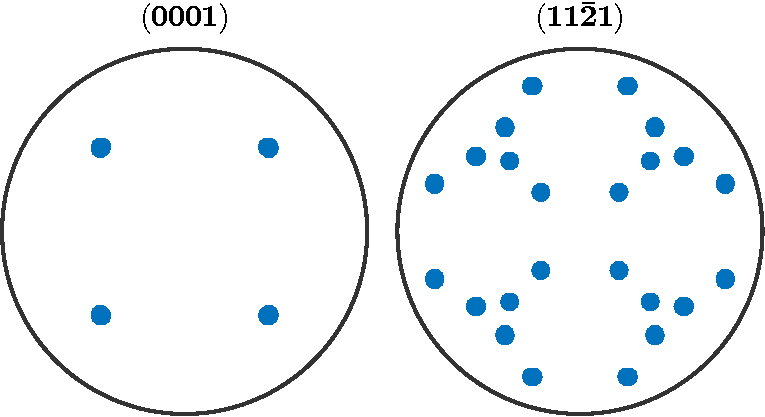
\includegraphics[height=3cm]{pic/HemPDF111.pdf}
    \quad
    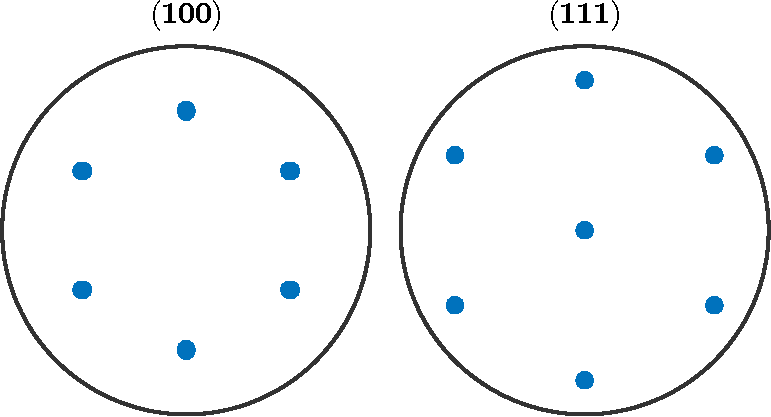
\includegraphics[height=3cm]{pic/MagPDF110.pdf}
  \end{center}
\end{onlyenv}

\end{overlayarea}
\end{frame}


\subsection*{phase transistion III}

\begin{frame}[fragile]
  \frametitle{Relationship Between Lattice Planes}

  \begin{overlayarea}{\textwidth}{8cm}

  Problem: compute the minimal angle between two lattice planes of two
  different grains having different orientation and different phase.
 \begin{lstlisting}[style=input]
m_Mag = Miller(1,0,0,cs_Magnetite);
m_Hem = Miller(1,1,-2,0,cs_Hematite);
 \end{lstlisting}
  \begin{onlyenv}<1>
    \vspace{-.3cm}
    \begin{lstlisting}[style=output]
m_Mag = /+Miller+/ (show methods, plot)
 size: 1 x 1
 mineral: Magnetite (432)
  h 1
  k 0
  l 0

m_Hem = Miller (show methods, plot)
 size: 1 x 1
 mineral: Hematite (321, X||a*, Y||b, Z||c)
  h  1
  k  1
  i -2
  l  0
\end{lstlisting}
  \end{onlyenv}

  \pause
  \medskip

  The orientation relation should be given by
  \begin{lstlisting}[style=input]
Mag2Hem = orientation('map',...
  Miller(1,1,1,CS_Mag),Miller(0,0,0,1,CS_Hem),...
  Miller(-1,0,1,CS_Mag),Miller(1,0,-1,0,CS_Hem))
  \end{lstlisting}
  \begin{onlyenv}<2>
    \vspace{-0.3cm}
    \begin{lstlisting}[style=output]
Mag2Hem = /+misorientation+/ (show methods, plot)
  size: 1 x 1
  crystal symmetry : Magnetite (m-3m)
  crystal symmetry : Hematite (-3m1, X||a*, Y||b, Z||c)

  Bunge Euler angles in degree
  phi1 Phi phi2 Inv.
  120 54.7356 45 0
    \end{lstlisting}
  \end{onlyenv}

  \pause
  \medskip

  The minimum angle
  \begin{lstlisting}[style=input]
min(angle(Mag2Hem * m_Mag.symmetrise,m_Hem ))/degree
 \end{lstlisting}
  \begin{onlyenv}<3>
    \vspace{-.3cm}
    \begin{lstlisting}[style=output]
  35.2644
    \end{lstlisting}
  \end{onlyenv}

\end{overlayarea}

\end{frame}

\section{Misorientation Space}

\subsection*{one axis}

\begin{frame}[fragile]
  \frametitle{The Misorientation Space - Disjoint Symmetries}

  \begin{columns}
    \begin{column}{0.6\textwidth}
      \begin{lstlisting}[style=input]
plot(orientationRegion)
      \end{lstlisting}

      \pause
      \begin{lstlisting}[style=input]
cs3 = crystalSymmetry('3')
oR  = orientationRegion(cs3)
plot(oR,'color','r')
\end{lstlisting}

      \pause
      \begin{lstlisting}[style=input]
cs4 = crystalSymmetry('4')
oR  = orientationRegion(cs4)
plot(oR,'color','g')
      \end{lstlisting}

      \pause
      \begin{lstlisting}[style=input]
oR = orientationRegion(cs3,cs4)
plot(oR,'color','r')
      \end{lstlisting}

      \pause

      \begin{onlyenv}<5>
        \begin{lstlisting}[style=input]
cs2 = crystalSymmetry('211')
oR = orientationRegion(cs3,cs2)
plot(oR,'color','r')
        \end{lstlisting}
      \end{onlyenv}

      \begin{onlyenv}<6>
        \begin{lstlisting}[style=input]
cs2 = crystalSymmetry('222')
oR = orientationRegion(cs3,cs2)
plot(oR,'color','r')
        \end{lstlisting}
      \end{onlyenv}

    \end{column}
    \begin{column}{0.4\textwidth}
      \only<1>{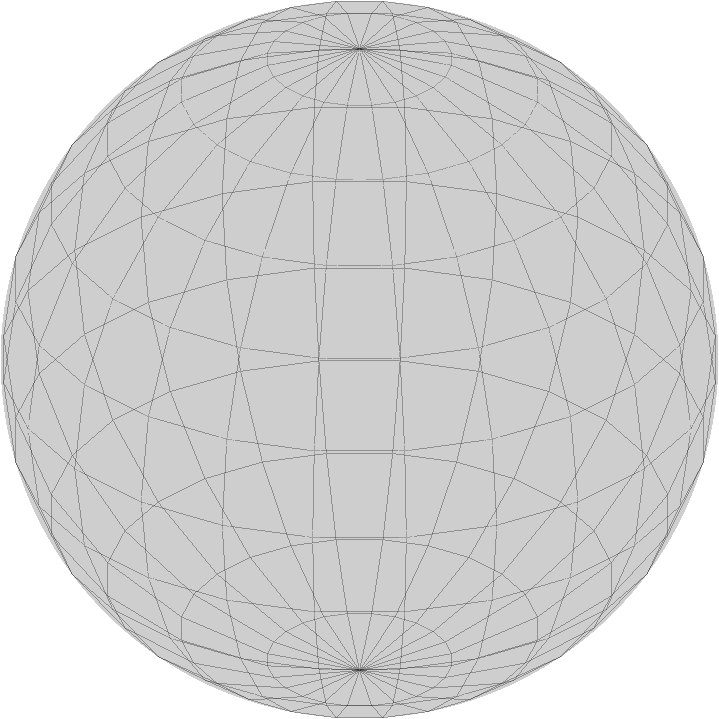
\includegraphics[width=\textwidth]{pic/oR1}}
      \only<2>{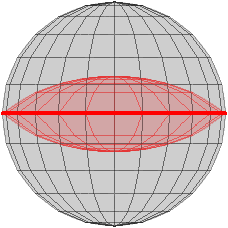
\includegraphics[width=\textwidth]{pic/oR3a}}
      \only<3>{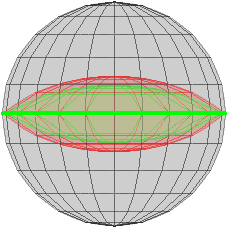
\includegraphics[width=\textwidth]{pic/oR4a}}
      \only<4>{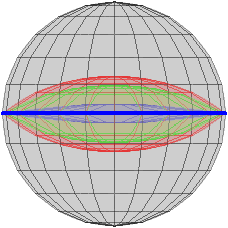
\includegraphics[width=\textwidth]{pic/oR12a}}
      \only<5>{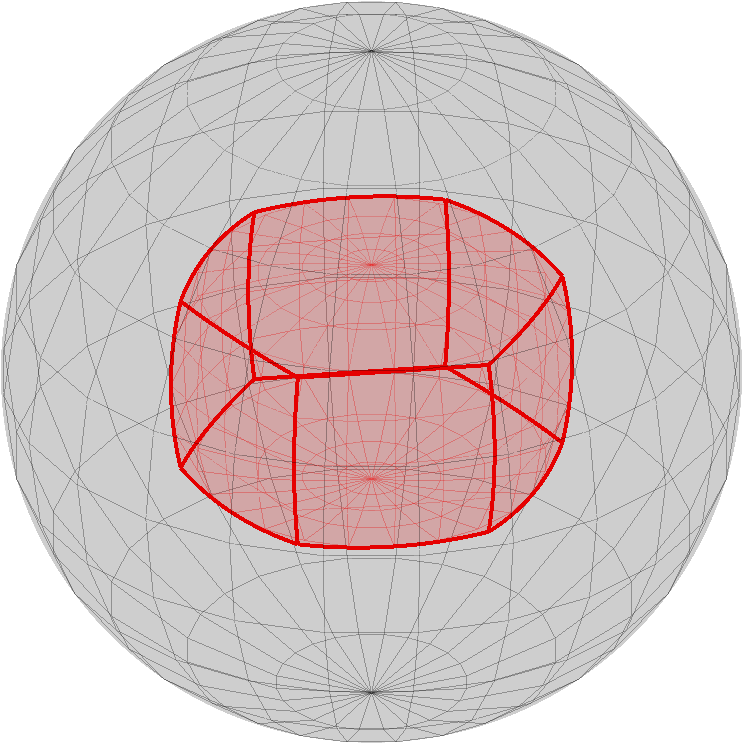
\includegraphics[width=\textwidth]{pic/oR321}}
      \only<6>{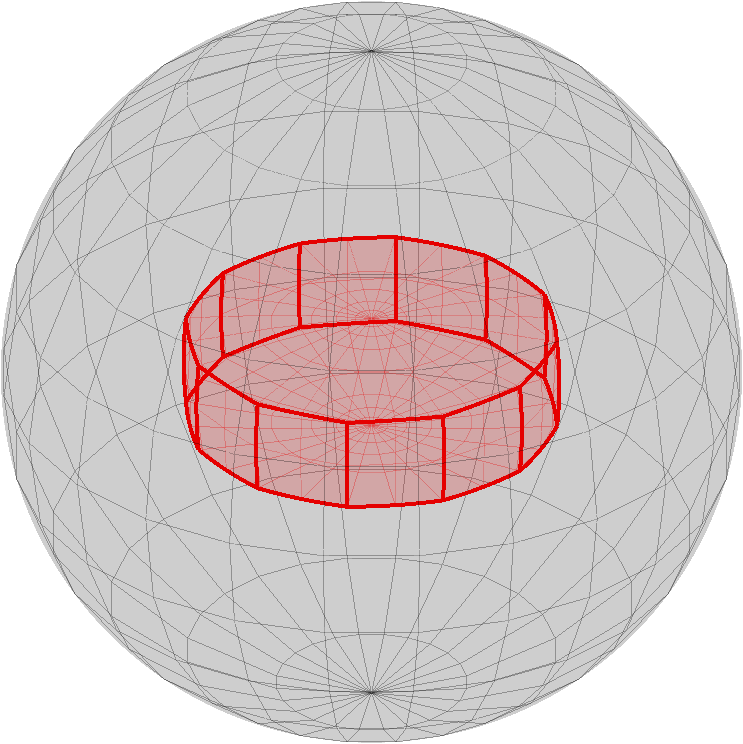
\includegraphics[width=\textwidth]{pic/oR622}}
    \end{column}
  \end{columns}
\end{frame}

\subsection*{common symmetries}

\begin{frame}[fragile]
  \frametitle{The Misorientation Space - Common Symmetries}

  \begin{columns}
    \begin{column}{0.6\textwidth}
      \begin{lstlisting}[style=input]
cs = crystalSymmetry('211')
oR = orientationRegion(cs,cs)
plot(oR,'color','r')
      \end{lstlisting}

      \pause
      \begin{lstlisting}[style=input]
cs = crystalSymmetry('3')
oR = orientationRegion(cs,cs)
\end{lstlisting}

      \pause
      \begin{lstlisting}[style=input]
cs = crystalSymmetry('222')
oR = orientationRegion(cs,cs)
      \end{lstlisting}
      \pause

      \begin{lstlisting}[style=input]
cs = crystalSymmetry('222')
oR = orientationRegion(cs,cs,...
     'antipodal')
      \end{lstlisting}

      \pause
      \begin{lstlisting}[style=input]
cs = crystalSymmetry('432')
oR = orientationRegion(cs)
      \end{lstlisting}


    \end{column}
    \begin{column}{0.4\textwidth}
      \only<1>{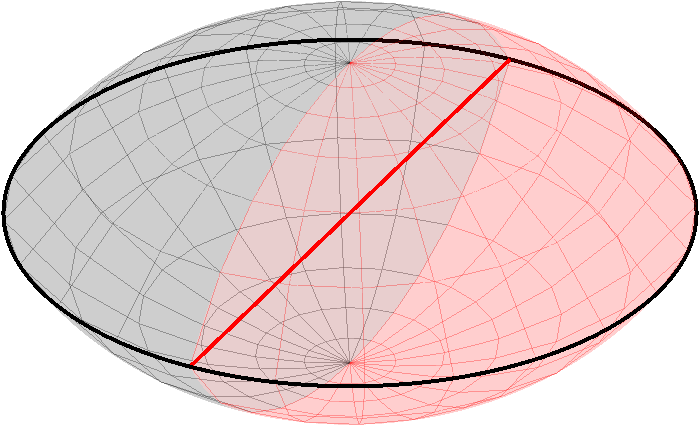
\includegraphics[width=\textwidth]{pic/oR22}}
      \only<2>{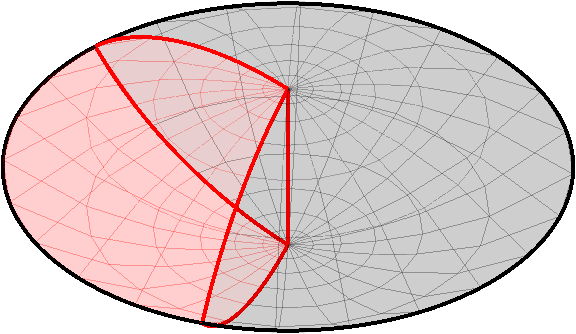
\includegraphics[width=\textwidth]{pic/oR33}}
      \only<3>{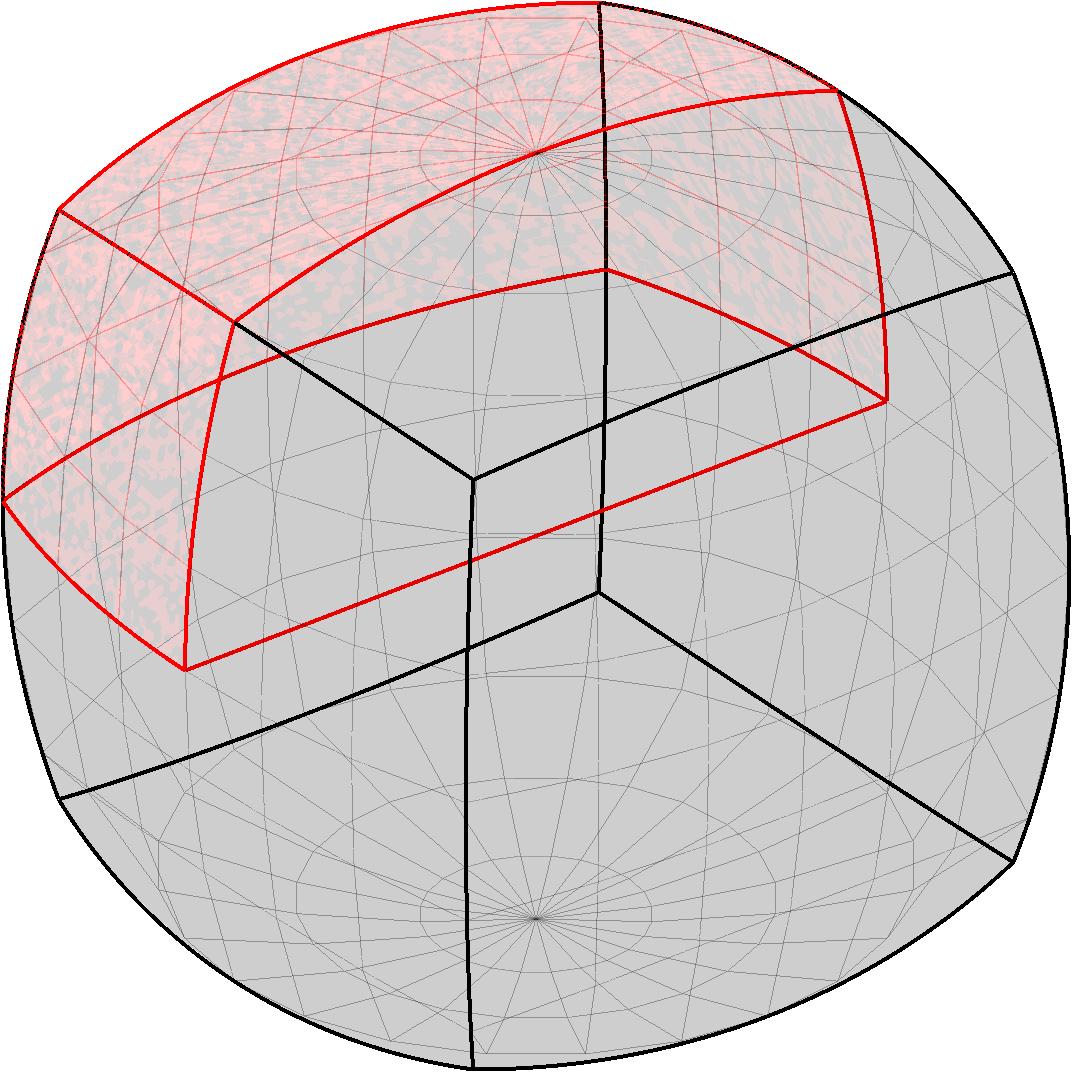
\includegraphics[width=\textwidth]{pic/oR2222}}
      \only<4>{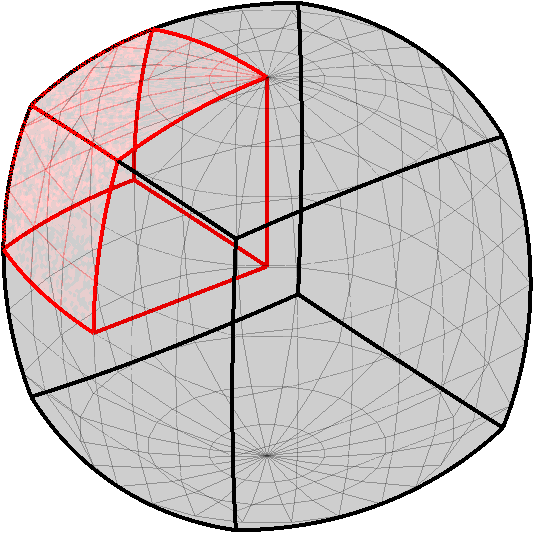
\includegraphics[width=\textwidth]{pic/oR2222a}}
      \only<5>{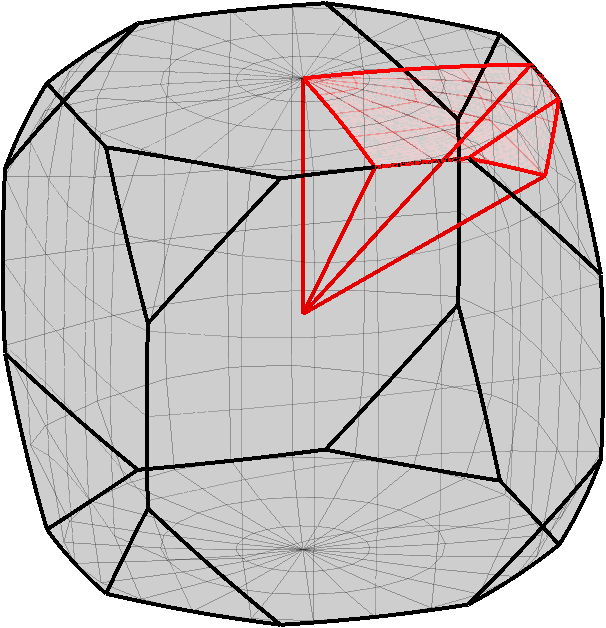
\includegraphics[width=\textwidth]{pic/oR4343}}
    \end{column}
  \end{columns}
\end{frame}


\subsection*{phase transitions}

\begin{frame}[fragile]
  \frametitle{The Misorientation Space - Phase Transitions}

  \begin{columns}
    \begin{column}{0.6\textwidth}
      \begin{lstlisting}[style=input]
cs1 = crystalSymmetry('23')
cs2 = crystalSymmetry('32')
oR = orientationRegion(cs1,cs2)
      \end{lstlisting}

      \pause
      \pause
      \begin{lstlisting}[style=input]
cs1 = crystalSymmetry('432')
cs2 = crystalSymmetry('321')
oR = orientationRegion(cs1,cs2)
\end{lstlisting}

      \pause
      \begin{lstlisting}[style=input]
Mag2Hem = orientation('map',...
   Miller(1,1,1,cs1), ...
   Miller(0,0,0,1, cs2) , ...
   Miller(-1,0,1, cs1), ...
   Miller(1,0,-1,0,cs2))
plot(Mag2Hem)
      \end{lstlisting}

      \pause
      \begin{lstlisting}[style=input]
plotSection(Mag2Hem)
\end{lstlisting}


    \end{column}
    \begin{column}{0.4\textwidth}
      \only<1>{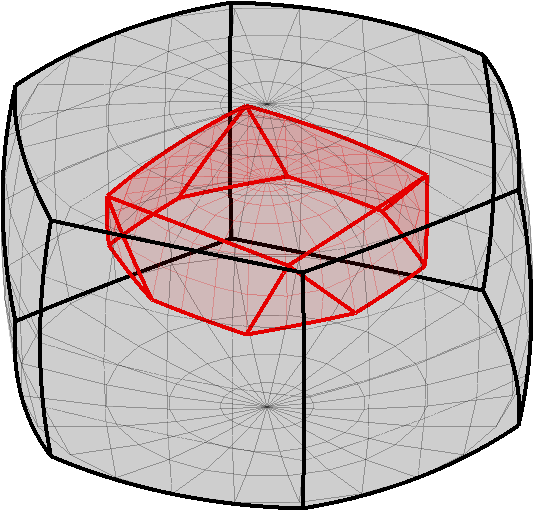
\includegraphics[width=\textwidth]{pic/oR2332a}}
      \only<2>{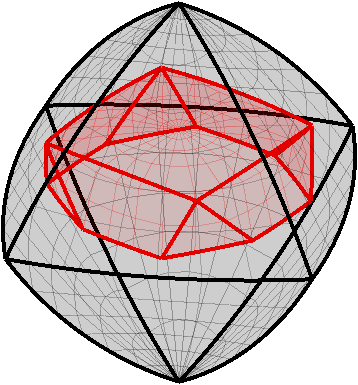
\includegraphics[width=\textwidth]{pic/oR2332b}}
      \only<3>{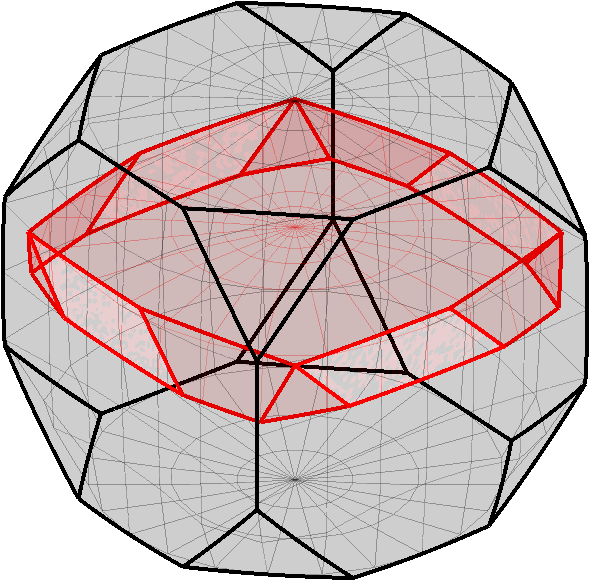
\includegraphics[width=\textwidth]{pic/oR43232a}}
      \only<4>{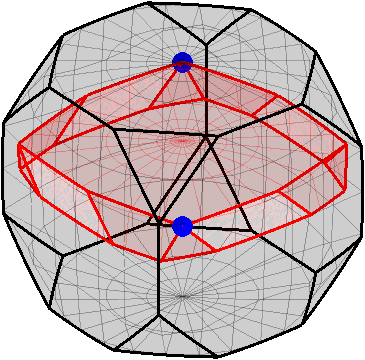
\includegraphics[width=\textwidth]{pic/oR43232b}}
      \only<5>{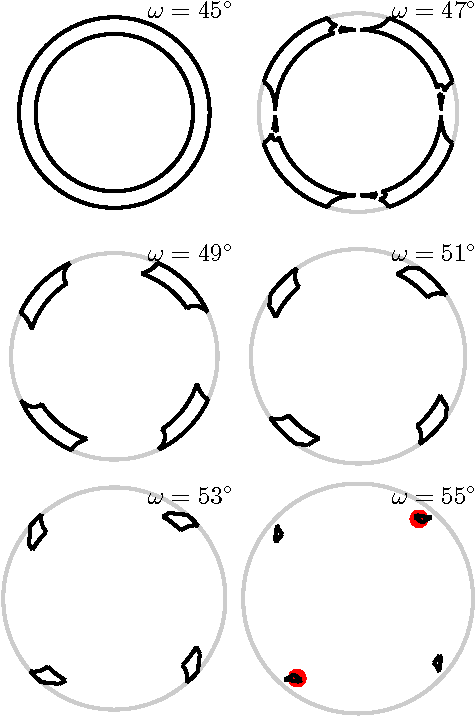
\includegraphics[width=\textwidth]{pic/oR43232Section}}
    \end{column}
  \end{columns}
\end{frame}



\section{Example}

\subsection{example}

\begin{frame}[fragile]
  \frametitle{Austenite to Martensite transition}

  \vspace{-0.6cm}
  \begin{overlayarea}{\textwidth}{0.61\textheight}
    \begin{columns}
      \begin{column}{0.6\textwidth}
        \begin{lstlisting}[style=input]
ebsd=loadEBSD('martensite.ctf')
        \end{lstlisting}
        \begin{onlyenv}<1>
          \vspace{-0.3cm}
          \begin{lstlisting}[style=output]
ebsd = /+EBSD+/ (show methods, plot)

 Phase  Orientations  Mineral Symmetry
     1    25389 (69)      fcc     m-3m
     2    1884 (5.1)      bcc     m-3m
     3     9693 (26)      hcp    6/mmm

 Properties: bands, bc, bs, error, mad
 Scan unit : um
          \end{lstlisting}
        \end{onlyenv}

        \pause

        \vspace{-0.3cm}
        \begin{lstlisting}[style=input]
grains=calcGrains(ebsd);
plot(grains.boundary)
gB=grains.boundary('fcc','hcp')
        \end{lstlisting}
        \begin{onlyenv}<2>
          \vspace{-0.3cm}
          \begin{lstlisting}[style=output]
gB = /+grainBoundary+/ (show methods, plot)

 Segments  mineral 1  mineral 2
     3829        fcc        hcp
          \end{lstlisting}
        \end{onlyenv}

      \pause
      \vspace{-0.3cm}
      \begin{lstlisting}[style=input]
plotSection(gB.misorientation)
      \end{lstlisting}

      \pause
      \vspace{-0.3cm}
      \begin{lstlisting}[style=input]
mdf=calcMDF(gB.misorientation)
plotSection(mdf)
      \end{lstlisting}

\pause
      \vspace{-0.3cm}
      \begin{lstlisting}[style=input]
plot(gB.misorientation,...
   mdf.eval(gB.misorientation))
      \end{lstlisting}

      \end{column}
\begin{column}{0.4\textwidth}
  \only<1>{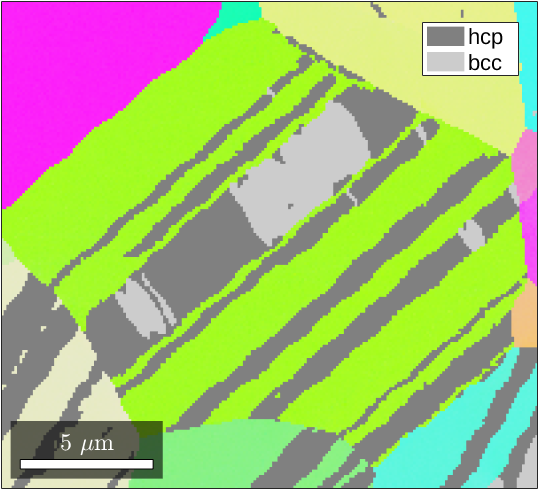
\includegraphics[width=\textwidth]{pic/twinRaw}}
  \only<2-3>{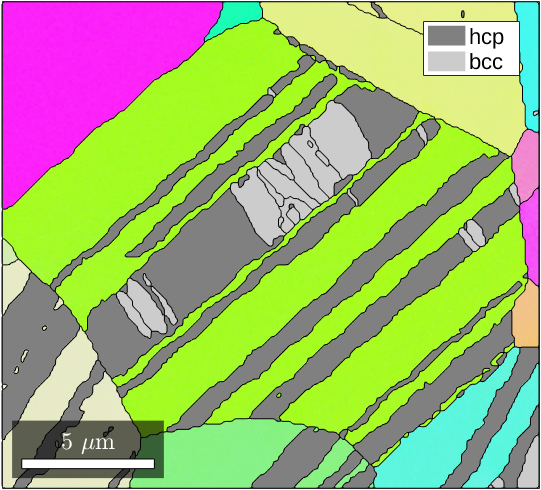
\includegraphics[width=\textwidth]{pic/twinGrains}}
  \begin{onlyenv}<4>
    \begin{lstlisting}[style=output]
mdf = /+MDF+/
  crystal sym: fcc (m-3m)
  crystal sym: hcp (6/mmm)

  Harmonic portion:
    degree: 38
    weight: 1
          \end{lstlisting}
        \end{onlyenv}
        \only<5>{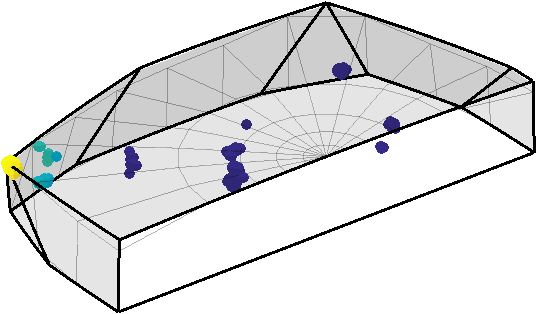
\includegraphics[width=\textwidth]{pic/oRTwin}}
\end{column}
\end{columns}

\end{overlayarea}

\begin{overlayarea}{\textwidth}{0.4\textheight}
  \only<3>{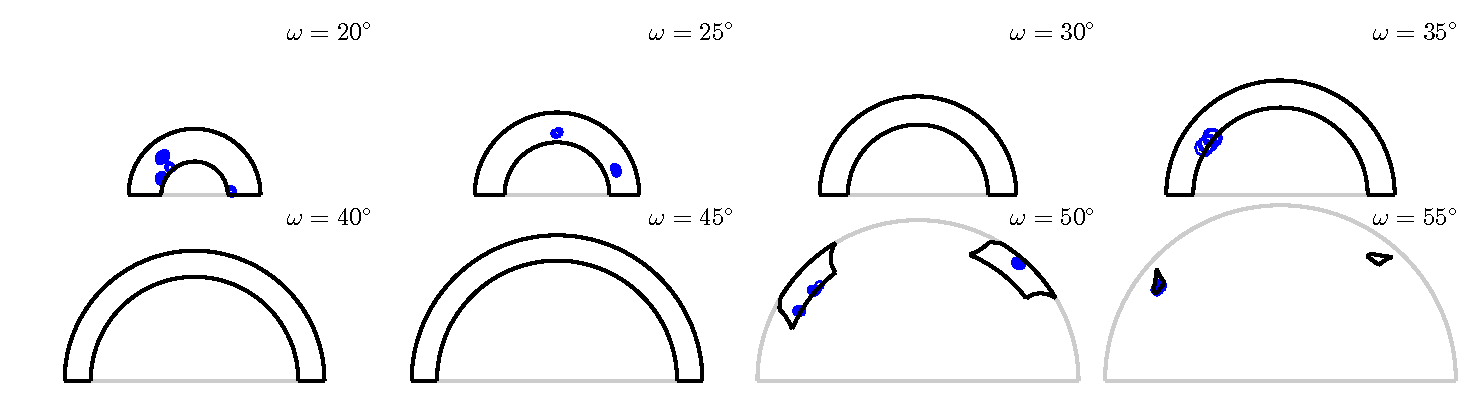
\includegraphics[width=\textwidth]{pic/twinSections}}
  \only<4-5>{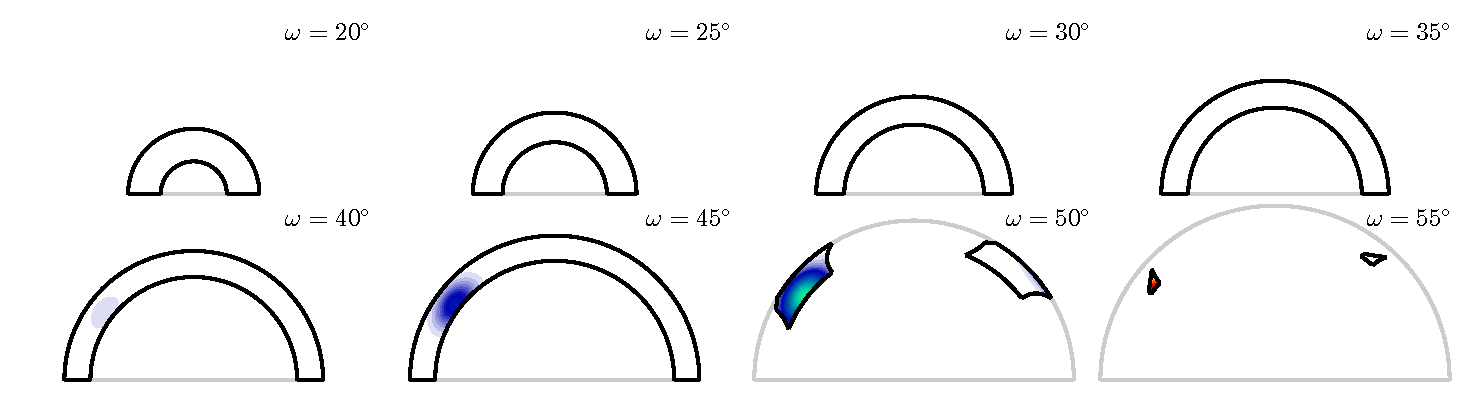
\includegraphics[width=\textwidth]{pic/MDFSections}}
\end{overlayarea}

\end{frame}

\subsection*{twinBoundaries}

\begin{frame}[fragile]
  \frametitle{Austenite to Martensite transition}

  \begin{columns}
    \begin{column}{0.67\textwidth}
      \vspace{-0.5cm}
      \begin{overlayarea}{\textwidth}{\textheight}
      \begin{lstlisting}[style=input]
plot(gB,gB.misorientation.angle)
      \end{lstlisting}

      \pause

      \vspace{-0.1cm}
      \begin{lstlisting}[style=input]
oR = fundamentalRegion(csFCC,csHCP)
mO = orientation(oR.V,csFCC,csHCP)
tB = gB(gB.isTwinning(mO,1*degree))
plot(tB,'lincecolor','r')
      \end{lstlisting}
      \begin{onlyenv}<2>
        \vspace{-0.3cm}
        \begin{lstlisting}[style=output]
tB = /+grainBoundary+/ (show methods, plot)

 Segments  mineral 1  mineral 2
     3283        fcc        hcp
           \end{lstlisting}
        \end{onlyenv}

      \pause

      \vspace{-0.1cm}
      \begin{lstlisting}[style=input]
[mGrains,parent] = merge(grains,tB)
plot(mGrains.boundary)
      \end{lstlisting}
        \begin{onlyenv}<3>
          \vspace{-0.3cm}
          \begin{lstlisting}[style=output]
mGrains = /+grain2d+/ (show methods, plot)

 Phase  Grains  Pixels  Mineral  Symmetry
     1       8    7156      fcc      m-3m
     2      26    1884      bcc      m-3m
     3       6   27926      hcp     6/mmm
           \end{lstlisting}
        \end{onlyenv}

        \pause

          \vspace{-0.1cm}
        \begin{lstlisting}[style=input]
wasFCC = parent(grains.phase==1);
mGrains.phase(wasFCC) = 1
      \end{lstlisting}
        \begin{onlyenv}<4>
          \vspace{-0.3cm}
          \begin{lstlisting}[style=output]
mGrains = /+grain2d+/ (show methods, plot)

 Phase  Grains  Pixels  Mineral  Symmetry
     1      13   35079      fcc      m-3m
     2      26    1884      bcc      m-3m
     3       1       3      hcp     6/mmm
           \end{lstlisting}
        \end{onlyenv}

      \end{overlayarea}
    \end{column}
    \begin{column}{0.35\textwidth}
      \vspace{-0.5cm}
      \only<1>{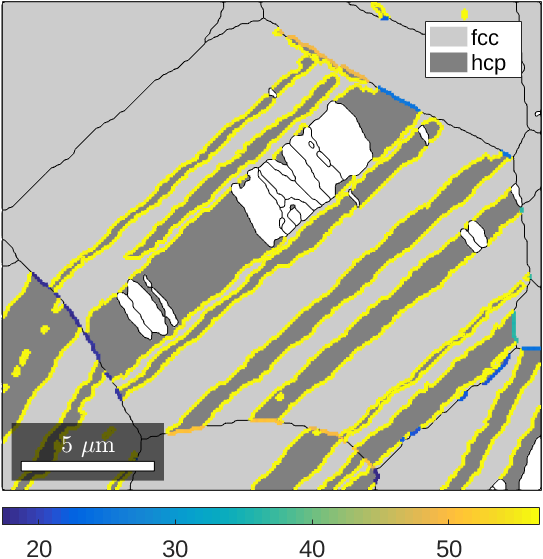
\includegraphics[width=\textwidth]{pic/gBAngle.png}}
      \only<2>{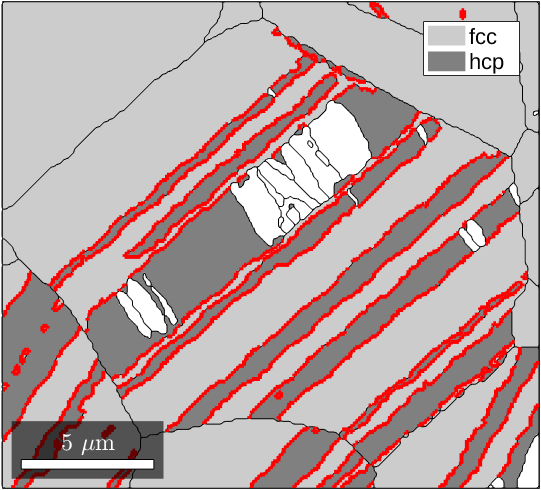
\includegraphics[width=\textwidth]{pic/twinBoundary}}
      \only<3>{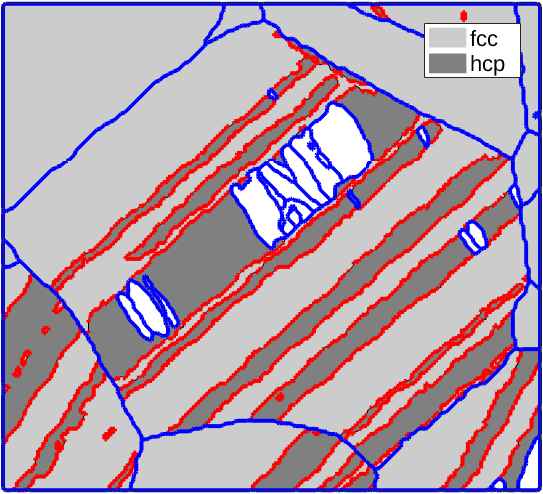
\includegraphics[width=\textwidth]{pic/grainMerged}\\
        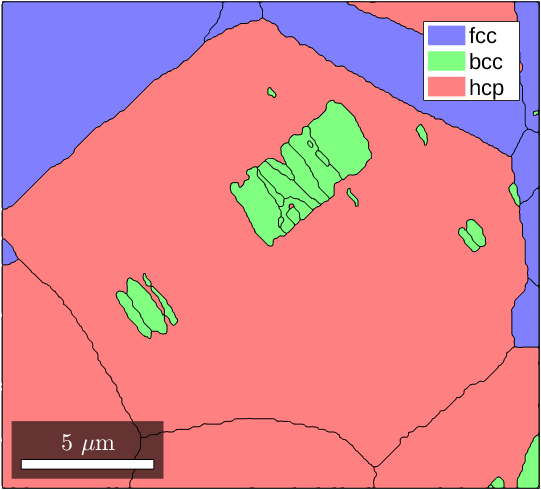
\includegraphics[width=\textwidth]{pic/grainMergeda}}
      \only<4>{
        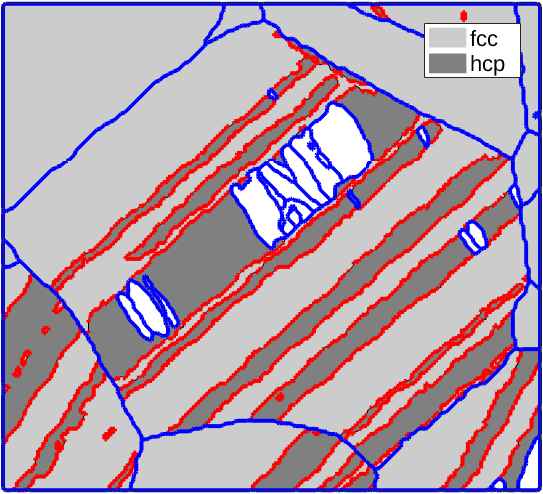
\includegraphics[width=\textwidth]{pic/grainMerged}\\
        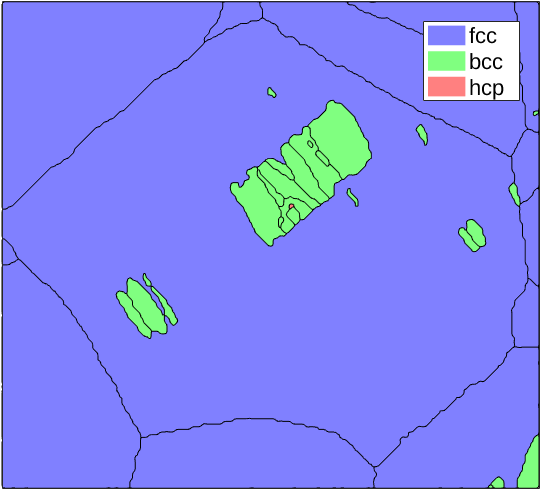
\includegraphics[width=\textwidth]{pic/grainMergedb}}
    \end{column}
  \end{columns}
\end{frame}



\section{Angle Distributions}

\subsection*{Angle Histograms}

\begin{frame}[fragile]
  \frametitle{Misorientation angel and axis}

  \begin{overlayarea}{\textwidth}{0.55\textheight}

    the smallest rotational angle of all symmetrically equivalent
    misorientations to \textbf{MO} is called \structure{misorientation angle}
    \vspace{-.2cm}
    \begin{lstlisting}[style=input]
angle(O1,O2), angle(MO), angle(inv(MO))
    \end{lstlisting}

\pause

for boundary misorientations we can do a simple statistics by
\vspace{-.2cm}
    \begin{lstlisting}[style=input]
gB = grain.boundary
hist(gB('fcc','fcc').misorientation.angle ./ degree)
    \end{lstlisting}

    \pause

    nicer  plots
    \vspace{-.2cm}
    \begin{lstlisting}[style=input]
plotAngleDistribution(gB('fcc','fcc').misorientation)
    \end{lstlisting}



  \end{overlayarea}

  \begin{overlayarea}{\textwidth}{0.45\textheight}
    \centering
    \only<2>{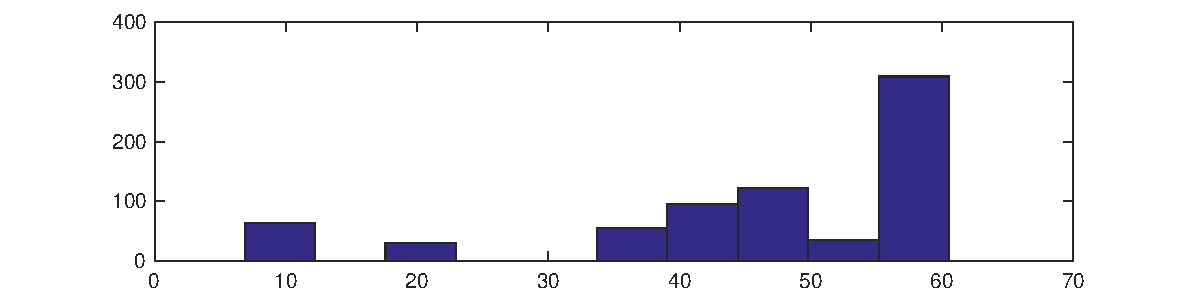
\includegraphics[width=\textwidth]{pic/histAngleSimple}}
    \only<3>{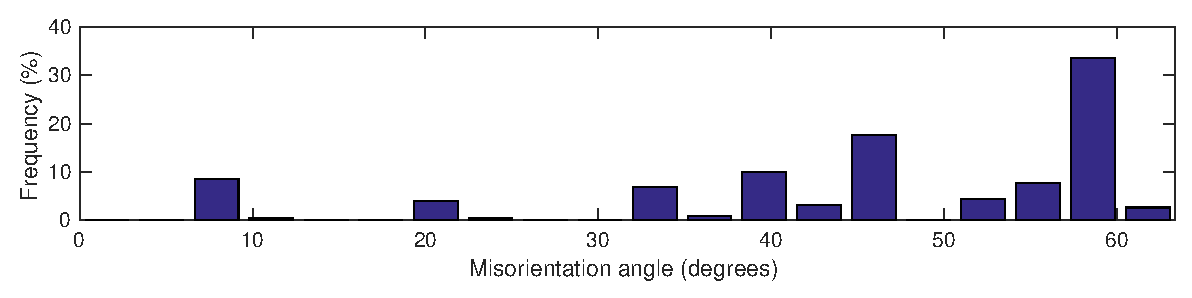
\includegraphics[width=\textwidth]{pic/histAngle}}
  \end{overlayarea}

\end{frame}


\subsection*{Angle Distributions}

\begin{frame}[fragile]
  \frametitle{Angle Distributions}

   \begin{overlayarea}{\textwidth}{0.55\textheight}
%     Angle histograms for several phases
%     \vspace{-.2cm}
%     \begin{lstlisting}[style=input]
% plotAngleDistribution(gB('fcc','fcc').misorientation)
%     \end{lstlisting}
% hold on
% plotAngleDistribution(gB('fcc','hcp').misorientation)
% plotAngleDistribution(gB('bcc','hcp').misorientation)
% hold off
%    \pause

    The untextured, uncorrelated angle distribution
    \vspace{-.2cm}
    \begin{lstlisting}[style=input]
plotAngleDistribution(csFCC,csFCC)
    \end{lstlisting}

    \pause
    The textured, uncorrelated angle distribution
    \vspace{-.2cm}
    \begin{lstlisting}[style=input]
odfFCC = calcODF(ebsd('fcc').orientations);
mdf = calcMDF(odfFCC,odfFCC)
plotAngleDistribution(mdf)
\end{lstlisting}

\pause
    The textured, correlated angle distribution
    \vspace{-.2cm}
    \begin{lstlisting}[style=input]
mdf = calcMDF(gB('fcc','fcc').misorientation)
plotAngleDistribution(mdf)
\end{lstlisting}

  \end{overlayarea}

  \begin{overlayarea}{\textwidth}{0.4\textheight}
    \centering
    \only<1>{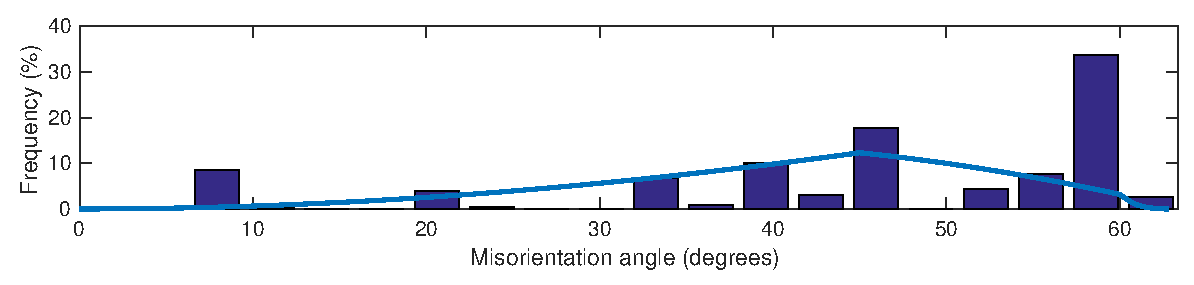
\includegraphics[width=\textwidth]{pic/angleDistriUniform}}
    \only<2>{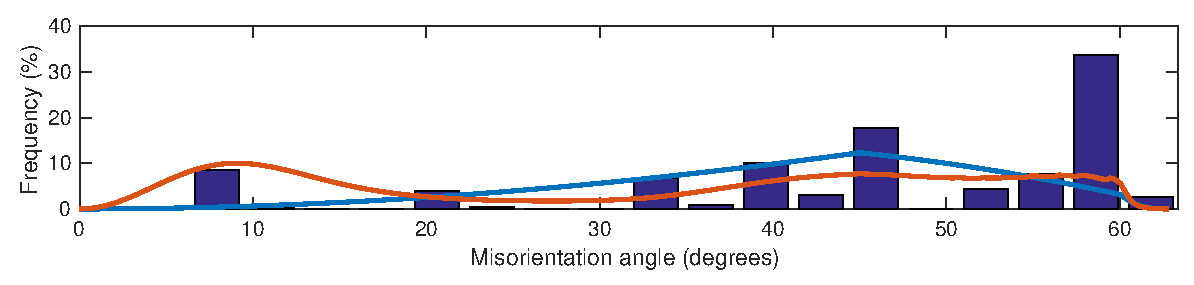
\includegraphics[width=\textwidth]{pic/angleDistriMDF1}}
    \only<3>{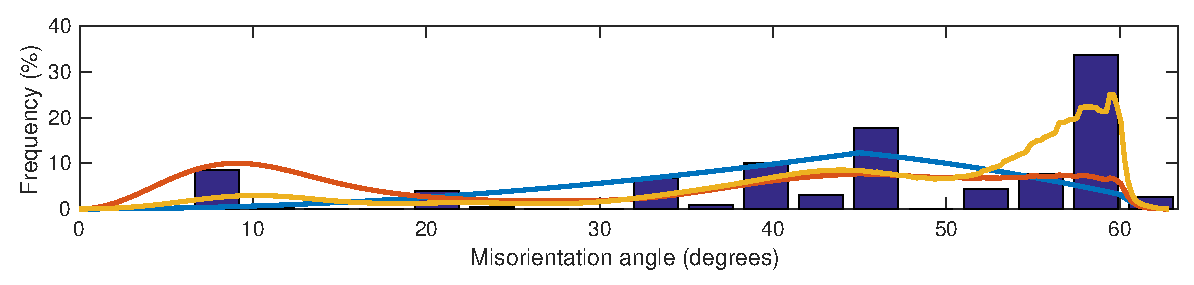
\includegraphics[width=\textwidth]{pic/angleDistriMDF2}}
  \end{overlayarea}


\end{frame}

%\subsection*{Statistics}

% \begin{frame}[fragile]
%   \frametitle{Misorientation Statistics}

%   \begin{columns}
%     \begin{column}{8cm}
%       \begin{lstlisting}[style=input]
% plotAngleDistribution(MO)
% hold on
% plotAngleDistribution(MO.CS)
% hold off
%       \end{lstlisting}

%       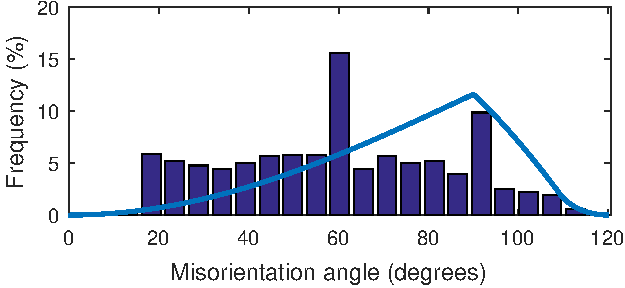
\includegraphics[width=\textwidth]{pic/angleDistri}

%       \pause

%   \begin{lstlisting}[style=input]
% plotAxisDistribution(MO)
%   \end{lstlisting}

%   \pause
% \vspace{-0.3cm}
%   \begin{lstlisting}[style=input]
% plotAxisDistribution(MO,'contourf')
%   \end{lstlisting}
% \end{column}
% \begin{column}{4cm}
%   \begin{overlayarea}{\textwidth}{8cm}
%     \begin{onlyenv}<2->
%       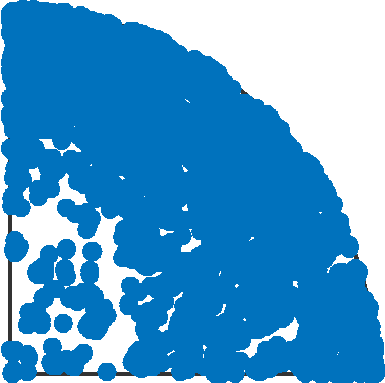
\includegraphics[width = \textwidth]{pic/axisDistri}
%     \end{onlyenv}

%     \medskip

%     \begin{onlyenv}<3>
%       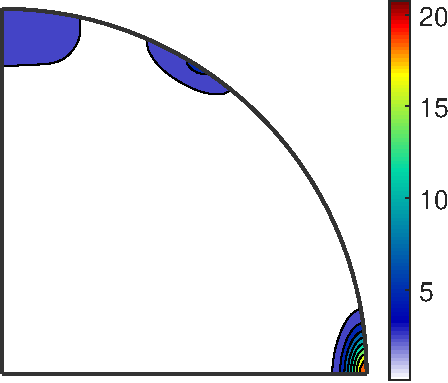
\includegraphics[width = \textwidth]{pic/axisDistriSmooth}
%     \end{onlyenv}
%   \end{overlayarea}

% \end{column}

% \end{columns}

% \end{frame}


\section{Axis Distribution}

\subsection*{axis in crystal}

\begin{frame}[fragile]
  \frametitle{Misorientation axis in crystal coordinates}


\begin{columns}

  \begin{column}{0.67\textwidth}
  \begin{overlayarea}{\textwidth}{\textheight}
    the misorientation realizing the minimum angle is
    \vspace{-0.2cm}
    \begin{lstlisting}[style=input]
MO.project2FundamentalRegion
    \end{lstlisting}
\begin{onlyenv}<1>
  \vspace{-.3cm}
  \begin{lstlisting}[style=output]
MO = /+misorientation+/ (show methods, plot)
  size: 1 x 1
  crystal symmetry : Magnetite (m-3m)
  crystal symmetry : Hematite (-3m1)

  Bunge Euler angles in degree
     phi1     Phi    phi2    Inv.
  60.1624 54.6037 314.719       0
\end{lstlisting}
\end{onlyenv}

\pause

  its rotational axis is the \structure{misorientation axis}
  \vspace{-0.2cm}
\begin{lstlisting}[style=input]
axis(MO)
\end{lstlisting}
\vspace{-.3cm}

  \begin{onlyenv}<2>
\begin{lstlisting}[style=output]
ans = /+Miller+/ (show methods, plot)
 size: 1 x 1
 mineral: Hematite (-3m1)
  h  0.6191
  k  3.8882
  i -4.5073
  l  3.3513
\end{lstlisting}
\end{onlyenv}

\pause


\begin{lstlisting}[style=input]
axis(inv(MO))
\end{lstlisting}
\vspace{-.3cm}
    \begin{onlyenv}<3>
\begin{lstlisting}[style=output]
ans = /+Miller+/ (show methods, plot)
 size: 1 x 1
 mineral: Magnetite (m-3m)
  h  4.9324
  k -6.4797
  l  2.0431
\end{lstlisting}
\end{onlyenv}

\pause
\begin{lstlisting}[style=input]
plotAxisDistribution(...
  gB.misorientation)
plotAxisDistribution(...
  inv(gB.misorientation))
\end{lstlisting}

\pause
\begin{lstlisting}[style=input]
plotAxisDistribution(...
  gB.misorientation,'contourf')
plotAxisDistribution(...
 inv(gB.misorientation),'contourf')
\end{lstlisting}
\end{overlayarea}
\end{column}
\begin{column}{0.33\textwidth}

  \begin{overlayarea}{\textwidth}{\textheight}
    \only<2-3>{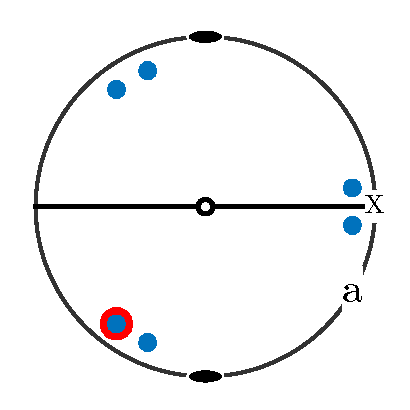
\includegraphics[width=\textwidth]{pic/misAxisa}}

    \only<3>{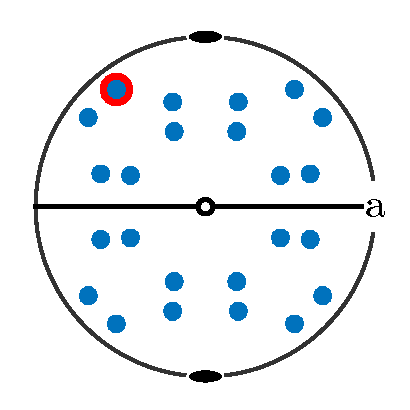
\includegraphics[width=\textwidth]{pic/misAxisb}}
    \begin{onlyenv}<4>
      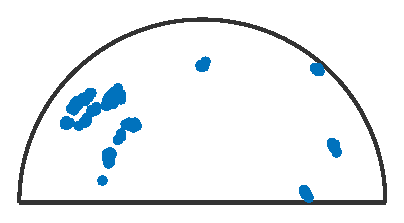
\includegraphics[width=\textwidth]{pic/AxisDistri1}

      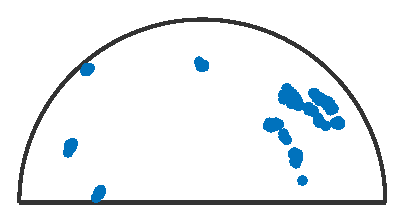
\includegraphics[width=\textwidth]{pic/AxisDistri2}
    \end{onlyenv}

    \begin{onlyenv}<5>
      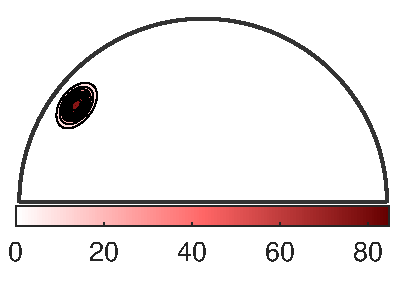
\includegraphics[width=\textwidth]{pic/AxisDistri3}

      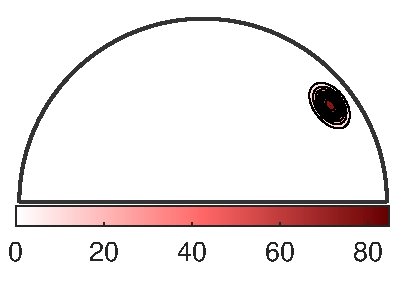
\includegraphics[width=\textwidth]{pic/AxisDistri4}
    \end{onlyenv}
  \end{overlayarea}
\end{column}
\end{columns}

\end{frame}


\subsection*{axis distributions}

\begin{frame}[fragile]
  \frametitle{Misorientation axis distributions}


\begin{columns}

  \begin{column}{0.67\textwidth}
    \begin{overlayarea}{\textwidth}{\textheight}

      The untextured, uncorrelated axis distribution
      \vspace{-0.2cm}
    \begin{lstlisting}[style=input]
plotAxisDistribution(csHCP,csFCC)
\end{lstlisting}

\pause

The textured, correlated axis distribution
\vspace{-0.2cm}
\begin{lstlisting}[style=input]
mdf = calcMDF(gB.misorientations)
plotAxisDistribution(mdf)
\end{lstlisting}
\begin{onlyenv}<2>
  \vspace{-0.3cm}
  \begin{lstlisting}[style=output]
mdf = /+MDF+/ (show methods, plot)
  crystal symmetry : fcc (m-3m)
  crystal symmetry : hcp (6/mmm)

  Harmonic portion:
    degree: 58
    weight: 1
\end{lstlisting}
\end{onlyenv}
\pause

\begin{lstlisting}[style=input]
[value,mori] = max(mdf)
plot(mori.axis)
\end{lstlisting}
\begin{onlyenv}<3>
  \vspace{-0.3cm}
\begin{lstlisting}[style=output]
value =
  232.1792

mori = /+misorientation+/ (show methods, plot)
  size: 1 x 1
  crystal symmetry : fcc (m-3m)
  crystal symmetry : hcp (6/mmm)

  Bunge Euler angles in degree
     phi1     Phi    phi2    Inv.
  210.936 54.7028 134.957       0
\end{lstlisting}
\end{onlyenv}
\pause

The textured, uncorrelated axis distribution
\vspace{-0.2cm}
\begin{lstlisting}[style=input]
mdf = calcMDF(odfFCC,odfHCP)
plotAxisDistribution(mdf)
\end{lstlisting}
\begin{lstlisting}[style=output]

\end{lstlisting}

  \end{overlayarea}
\end{column}
\begin{column}{0.31\textwidth}
  \begin{overlayarea}{\textwidth}{\textheight}
    \only<1-2>{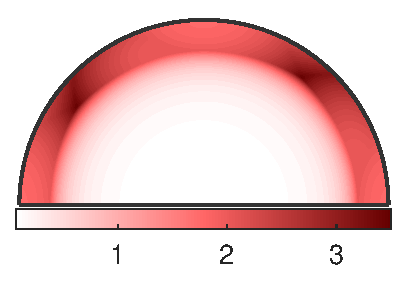
\includegraphics[width=\textwidth]{pic/mdfAxis}}
    \only<3->{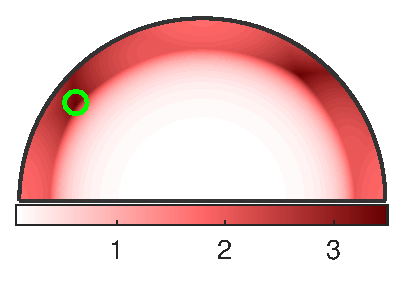
\includegraphics[width=\textwidth]{pic/mdfAxisM}}

    \only<2>{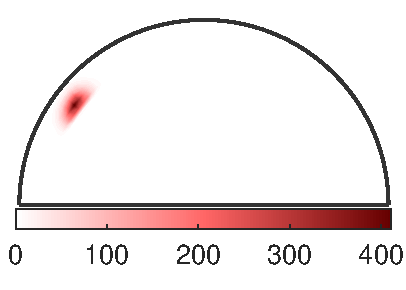
\includegraphics[width=\textwidth]{pic/mdfAxis3}}
    \only<3->{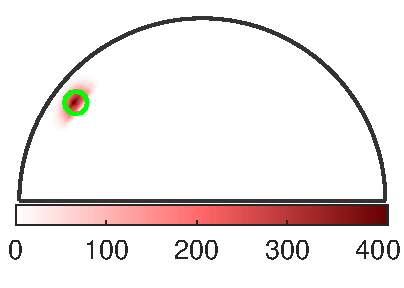
\includegraphics[width=\textwidth]{pic/mdfAxis3M}}

    \only<4>{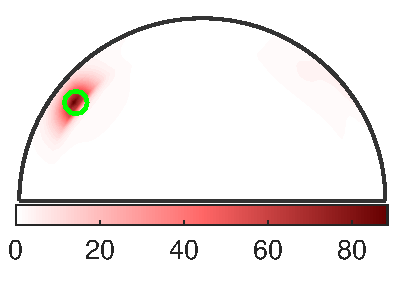
\includegraphics[width=\textwidth]{pic/mdfAxis4M}}
  \end{overlayarea}

\end{column}
\end{columns}
\end{frame}

\subsection*{axis in specimen}

\begin{frame}[fragile]
  \frametitle{Misorientation axis in specimen coordinates}

  \vspace{-.5cm}
  \begin{overlayarea}{\textwidth}{\textheight}

\begin{columns}

  \begin{column}{0.67\textwidth}


    Surprisingly the misorientation axis in specimen coordinates is unique
\begin{lstlisting}[style=input]
axis(O1,O2)
\end{lstlisting}

\begin{onlyenv}<1>
  \vspace{-.3cm}
\begin{lstlisting}[style=output]
ans = /+vector3d+/ (show methods, plot)
 size: 1 x 1
          x         y         z
  0.0495585  0.992437 -0.112305
\end{lstlisting}
\end{onlyenv}

\pause

\begin{lstlisting}[style=input]
[grains, ebsd.grainId] = ...
  calcGrains(ebsd)
\end{lstlisting}

\pause

\begin{lstlisting}[style=input]
gB = grains.boundary('fcc','hcp')
ids = gB.ebsdId;
oFCC = ebsd(ids(:,1)).orientations
oHCP = ebsd(ids(:,2)).orientations
\end{lstlisting}

\pause

\begin{lstlisting}[style=input]
plotAxisDistribution(oFCC,oHCP)
\end{lstlisting}

\pause

\begin{lstlisting}[style=input]
plotAxisDistribution(oFCC,oHCP,...
  'contourf')
\end{lstlisting}

\end{column}
  \begin{column}{0.33\textwidth}
    \only<1>{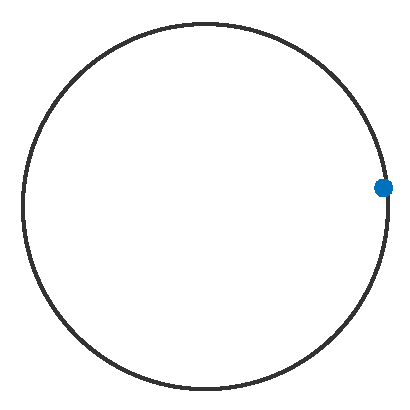
\includegraphics[width=\textwidth]{pic/misAxisc}}
    \only<4>{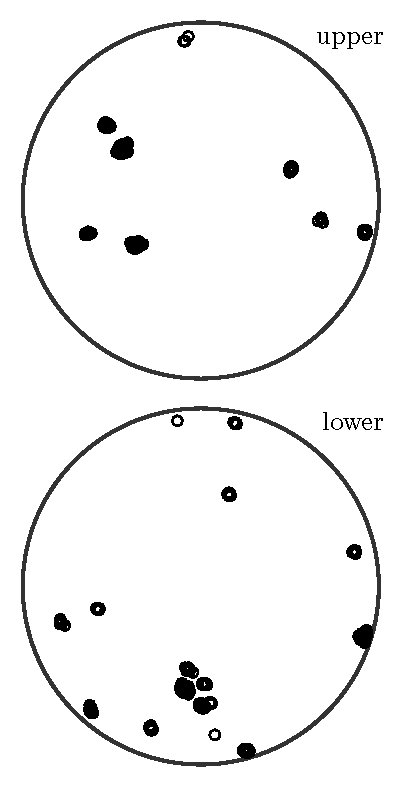
\includegraphics[width=\textwidth]{pic/AxisSample1}}
    \only<5>{\includegraphics[width=\textwidth]{pic/AxisSample2}}
  \end{column}

\end{columns}
\end{overlayarea}
\end{frame}

% \section{Exercises}

% \subsection*{Exercises2}

% \begin{frame}

%   \begin{Exercise}
%     Consider trigonal crystal symmetry.

%   \begin{enumerate}[a)]
%     \item Find all crystallographic directions symmetrically equivalent to $h
%       = (1, 0, \bar 1, 0)$ (Miller indices)!
%     \item Find crystallographic directions such that the number of their
%       crystallographic equivalent directions on the upper hemisphere (without
%       equator) is 1, 3, and 6, when including antipodal symmetry!
%     \item Consider the orientation given by the Euler angles $(30\degree,
%       90\degree, 90\degree)$ in Bunge convention. Give the Euler angles of
%       all symmetrically equivalent orientations!
%     \item Which positions in the (0,0,0,1) - pole figure corresponds to the
%       above orientation. Which crystal direction is rotated by this
%       orientation to the specimen direction (0,0,1)?
%     \item Construct an orientation that rotates the crystallographic
%       directions $(0,0,0,1)$ and $(2,\bar 1,\bar 1,0)$ onto the specimen
%       directions $(1,0,0)$ and $(0,1,0)$, respectively. Describe the rotation
%       by axis and angle.
%     \end{enumerate}

%   \end{Exercise}

% \end{frame}

\end{document}


% \begin{frame}[fragile]
% \begin{lstlisting}[mathescape=true]
% rot = rotation('Euler',$\phi_1$,$\Phi$,$\phi_2$,'ZXZ')
% rot = rotation('Euler',$\alpha$,$\beta$,$\gamma$,'ABG')
% rot = rotation('axis',v,'angle',omega)
% rot = rotation('map',$u_1$, $v_1$, $u_2$, $v_2$) % $\mathbf{gu}_1=\mathbf{v}_1,\mathbf{gu}_2=\mathbf{v}_2$
% \end{lstlisting}

% \begin{columns}
%   \begin{column}{8.5cm}

%     Calculations:

% \begin{lstlisting}
% v = rot * u    % apply rot to u
% rot = rot1 * rot2
% \end{lstlisting}

%     Basic Functions:

% \begin{lstlisting}[mathescape=true]
% angle(rot), axis(rot)
% angle(rot1,rot2), inv(rot)
% [$\phi_1$,$\Phi$,$\phi_2$] = Euler(rot)
% [$\alpha$,$\beta$,$\gamma$] = Euler(rot,'ABG')
% \end{lstlisting}

%   \end{column}

%   \begin{column}{3cm}
%     \includegraphics[width=3cm]{pic/quaternion}
%   \end{column}

% \end{columns}
% \end{frame}


% \subsection*{Symmetry}
% \begin{frame}[fragile]
%   \frametitle{Crystal Symmetries - The \MTEX Class \texttt{\bf symmetry}}

%   Definition:

% \begin{lstlisting}
% S = symmetry('triclinic',[a,b,c],[alpha,beta,gamma])
% S = symmetry('-3m',[a,b,c],/+'X||a*'+/);
% S = symmetry('-3m',[a,b,c],'X||a','Z||c*');
% S = symmetry('O');
% \end{lstlisting}

% \medskip

% \begin{columns}
%   \begin{column}{8.5cm}

% Load Symmetry from CIF file:

% \begin{lstlisting}
% symmetry('quartz.cif')
% \end{lstlisting}

% \medskip

%     Basic Functions:

% \begin{lstlisting}
% symmetrise(v,S)
% symmetrise(rot,CS,SS)
% rotation(S)
% project2FundamentalRegion(v,CS)
% project2FundamentalRegion(rot,CS,SS)
% \end{lstlisting}
%   \end{column}

%   \begin{column}{3cm}
%     \includegraphics[width=3cm]{pic/sym}
%   \end{column}

% \end{columns}

% \end{frame}

% \subsection*{Miller}

% \begin{frame}[fragile]
%   \frametitle{Crystal Directions - The \MTEX Class \texttt{\bf Miller}}

%   Definition:

% \begin{lstlisting}
% m = Miller(u,v,w,CS,'uvw');
% m = Miller(h,k,i,l,CS,'hkl');
% m = [Miller(1,1,-2,3,CS),Miller(0,1,-1,0,CS)]
% \end{lstlisting}

% \medskip

% \begin{columns}
%   \begin{column}{8.5cm}

%     Calculations:

% \begin{lstlisting}
% h1 + h2
% rot * h     % apply rot on h
% \end{lstlisting}

%     \medskip

%     Basic Functions:

%     \begin{onlyenv}<1>
% \begin{lstlisting}
% eq(h1,h2), angle(h1,h2)
% symmetrise(h)  %get all equivalent
% plot([h1,h2],'all')
% \end{lstlisting}
%     \end{onlyenv}

% 	\end{column}

%   \begin{column}{3cm}
%     \includegraphics[width=3cm]{pic/miller}
%   \end{column}
% \end{columns}


% 	\begin{onlyenv}<2>

% 		\lstset{stringstyle=\color{red},emph={antipodal},emphstyle=\em\color{red}}

% \begin{lstlisting}
% get(h,'hkl')
% eq(h1,h2,`antipodal`), angle(h1,h2,`antipodal`)
% symmetrise(h,`antipodal`)
% plot([h1,h2],'all',`antipodal`)
% \end{lstlisting}


%     \end{onlyenv}


% \end{frame}



% \begin{frame}[fragile]
%   \frametitle{Orientations - The \MTEX Class \texttt{\bf orientation}}

% Definition:

% \begin{lstlisting}[mathescape=true]
% ori = orientation(rot,CS,SS)
% ori = orientation('Euler',$\phi_1$,$\Phi$,$\phi_2$,CS,SS)
% ori = orientation('Euler',$\alpha$,$\beta$,$\gamma$,'ABG',CS,SS)
% ori = orientation('Miller',[h k l],[u v w],CS,SS)
% ori = orientation('brass',CS,SS)
% \end{lstlisting}

% \begin{columns}
%   \begin{column}{8.5cm}

%     Calculations:

% \begin{lstlisting}
% r = ori * h, h = ori \ r
% ori = rot * ori
% \end{lstlisting}

%     Basic Functions:

% \begin{lstlisting}[mathescape=true]
% eq(ori1,ori2), angle(ori1,ori2)
% symmetrise(ori), angle(ori)
% project2FundamentalRegion(ori,ref_ori)
% [$\phi_1$,$\Phi$,$\phi_2$]  = Euler(ori)
% \end{lstlisting}

%   \end{column}

%   \begin{column}{3cm}
%     \includegraphics[width=3cm]{pic/quaternion}
%   \end{column}

% \end{columns}
% \end{frame}

2732626
